\chapter{Background}\label{C:back}

\section{Network packet}

\par Communication between computers is established through the means of physical connections and protcols overlaying on top of this. 
A widespread communication protocol is to break down each point of communication into discrete pieces called network packets.
These network packets contain many layers (Figure: \ref{fig:OSIModel}) of communication information.
Communication layers can be broken down into a few independent layers which hold specific purposes. 
Each layer contains information which can aid with transporting the information to the correct computer securely.
As each layer is independent, each higher layer does not affect the forthcoming layers.
High layers of the model are for purposes such as reliability of data and the data itself in the packet.
For the purposes of this project, an explanation of only the first three layers of the Open Systems Interconnection (OSI) model is concerned.

\begin{figure}[H]
    \begin{center}
        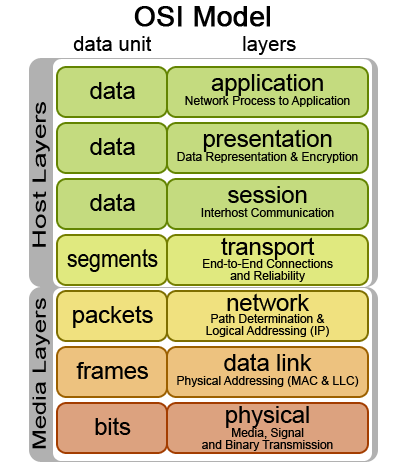
\includegraphics[width=5cm,height=5cm,keepaspectratio]{Images/OSIModel.png}
        \caption{OSI Model}
        \label{fig:OSIModel}
    \end{center}
\end{figure}

\subsection{Layer 1: Physical}

\par The physical layer is specifying the electrical and physical medium that is used to transport individual bits from one computer to another.
Two or more computers can be connected through many different physical mediums such as copper wiring and light fibers. 
Each medium has specific pros and cons, from implementation costs to throughtput capabilities.
The physical layer is responsible for transmitting and receiveing unstructured data.
Communication can be either Simplex, Half Duplex or Full Duplex.
The network topology is defined by how the physical layer is configured.
An example of a phyiscal medium is a copper medium is used to link two devices together.
This project will be investigating the latency present in a Gigabit Ethernet system, using copper based medium.

\subsection{Layer 2: Data link}

\par Data link layer is responsible for node-to-node data communication. 
It links from one device to another, determing the connection status of two physically connected devices.
A feature of this layer, is the ability to detect and correct errors created at the physical layer.
The IEEE Standard 802 \cite{IEEE802} details how this layer is split into two sub layers, Media Access Control (MAC), and Logical Link Control (LLC).
This project will cover networking switches which distinguish different destination devices by their unique MAC addresses.

\subsection{Layer 3: Network}

\par Network layer provides functionality when sending data across a network.
End-to-end communication is aided by assigning each node in the network an address, which it identifies itself with.
This allows data to be passed through intermediate nodes, which would continue to traverse until the target node has been reached.
This project will not be including this layer, or any others higher than this, as the latency measurements involved are short, single node-to-node distances.

\section{Network Latency}

\par As network operations are discretized, there is a delay between splitting data and information into pieces, then gathering this information again.
Each layer of the networking OSI model, a new piece of information is added to the discrete pieces.
The process of adding this information, and also removing it, causes delays in processing infromation.
The latency of a packet can be defined in many ways, for the purposes of this project, latency will be defined as the time from one node to another.

\subsection{Connection Time}

\par Connection time is defined to be the time that one end of a connection has been established with another end.
Only once the connection has been established, can information from one end flow to the other.
Many synchronization procedures and exchanging of information takes place when a link is brought up.
These procedure produces a delay, which can be measured to be the latency of a link.
This timing procedure is common for higher layered protocols, where security and authentication could be an issue.

\subsection{Round Trip Time}

\par Information sent from one place to another can be measured as time taken for a response to be sent from the other end of the link.
This can be measured by sending a packet from an end of a link, to the other requesting a response, and measuring the time taken for the response.
Half the round trip time can be inferred to be the latency of a link.

\section{Switching Techniques}

\par Network packet switches can switch network packets using different techniques.
Each technique has the ability to reduce packet latency, or increase reliability. 
Some techniques cannot work at all on specific data protocols.
Modern switches can achieve latency times ranging from hundreds of nanoseconds to tens of microseconds.
A big factor for the latency timing is how many transmitting devices are reaching the same reciever.

\subsection{Cut-Through}

\par Cut-Through switching is a latency reducing switching technique. 
Each transaction begins processing each network packet as soon as it is beginning to be transferred into the switch.
Once enough information is recieved to know which destination device it is, it begins forwarding information to the next hop.
This technique can only operate on data which has a header for the destination at the beginning of the packet.

\subsection{Store-and-Forward}

\par Switching data occasionally requires information which is embedded deep within the packet, hence header data cannot provide which device to transmit to.
A technique to process this data is called Store-and-Forward, where the whole packet is digested by the switch to determine the destination.
As this requires time to recieve data, process, then send this data, it does not have the same latency-reducing effect as Cut-Through does.

\section{Current Timing Solutions}

\par Timing of network packets can currently done through very expensive and bulky devices. 
For this reason, there are many software implementations that allow high speed packet processing.
The following software implementations have some restrictions on what hardware they can run on.
The precision to measure the latency of packets is unknown and needs to be investigated.
This project is to combine the flexibility of software and hardware to create a packet latency measurement utility.

\subsection{Data Plane Development Kit (DPDK)}

\par Data Plane Development Kit (DPDK) is a set of C libraries to allow for rapid processing of network packets.
It utilizes a few low level Application Programming Interfaces (APIs) to minimize the overhead of using a specific architecture computer.
Reducing this overhead of the CPU reduces the amount of latecy present in the act of measuring the time between packets itself.
This is a very good software solution to what is currently on the market, but one caveat to using this technology is that only specific hardware can be used.
The Network Interface Card (NIC) on the computer has to be compatible with the software.

\subsection{PF\textunderscore RING}

\par PF\textunderscore RING by ntop\texttrademark is a software solution for rapid network packet processing.
It is a network socket technology which improves the speed at which packets are captured by the processor.
Faster packet processing ensures that the time stamp placed on an ingress packet is accurate as it can be.
This is a software solution which could potentially work well, but is limited by the software latency of needing to be processed by a processor.
The NIC on the computer does not have to be a specific model, meaning this is a much more flexible solution.

\section{Field Programmable Gate Array(FPGA)}

\par Many implementations of measuring packet latency require processors and are limited to timing based off clock cycles from a processor.
Field Programmable Gate Array (FPGA) is a system of intertwined sets of logic gates, with configurable links between them.
This has the advantage of begin able to create complex digital circuits with no need for a clock signal.
This means no processor is involved with timing critical operations.
Timing is dependant on the speed of the input clock and the limitations of the Gate Array Fabric.

\subsection{Reconfigurable Macro Cells}

\par Sets of logic gates in a FPGA are called Macro Cells. 
These sets of logic gates are reconfigurable to select which logic operation takes place through the cell, and also what the inputs are.
Some Macro Cells have specific capabilities, such as the ability to generate a clock signal, or recieve a clock signal reliably.
Each Cell recieves information about configuration from Flash memory embedded on the board nearby.

\subsection{FPGA vs Microcontroller}
